\chapter{Clustering Functors}

\todo[talk about how this is a "rich" definition of clustering algorithms]

In this chapter we define a specific kind of functor which will be the object of study for the remainder of this report.



\section{Categories of Finite Metric Spaces}

\begin{definition}{Finite Metric Spaces}{}
We define three categories $\iso, \inj$ and $\gen$ all sharing the same objects:

\begin{equation*}
\ob(\M) := \{(X,d_X): \text{$X$ a finite set and $d_X$ a metric}\}
\end{equation*}

The three categories are distinguished by their morphisms. For $A, B \in \ob(\M)$ we define:
\begin{align*}
\mor_\gen(A,B) &:= \{f: A \to B: \text{$f$ distance non-increasing}\} \\
\mor_\inj(A,B) &:= \{f: A \to B: \text{$f$ distance non-increasing injective}\} \\
\mor_\iso(A,B) &:= \{f: A \to B: \text{$f$ isometry}\} \\
\end{align*}

\todo[format this better]
\end{definition}


By construction we have inclusions $\iso \subset \inj \subset \gen$. As we will see later that this can be seen as looking for different levels of invariances. Somewhere there exists a sweetspot of existence and richness \todo[better wording].


\begin{myremark}{Structure of $\iso$}{}
The structure of $\iso$ is perhaps the easiest to understand. We can consider the isometry classes of metric spaces. Then there exist morphisms between $A, B \in \ob(\iso)$ if and only they are in the same isometry class.

Thinking of morphisms as edges in a graph and the metric spaces as the edges we get a graph that consists of disjoint cliques.

\todo[clean up my ramblings]
\end{myremark}

\begin{myremark}{Structure of $\gen$}{}
The category $\gen$ is special in the sense that it most morphisms. Indeed for any $A,B \in \ob(\gen)$ non-empty there exists the morphism:
$$
\mathrm{const}_b: A \to B, \ a \mapsto b
$$
for some $b \in B$.
\end{myremark}

\todo[do the above remarks deserve a yellow border?]

\section{Partitions}
In this section we define some machinery that will be use to define the outputs of clustering schemes.

\begin{definition}{Partitions of Finite Sets}{}
Let $X$ be a finite set. A partition $P$ of $X$ is the set of equivalence classes $X/_{\sim_P}$ for some equivalence relation $\sim_P$ on $X$.
The set of all such partitions is denoted by $\P(X)$.
\end{definition}

\begin{myremark}{}{}
The above construction gives a bijection between the set of partitions $\P(X)$ and the equivalence relations on $X$. We will interchangeably use the notation $P$ as a partition and $\sim_P$ as the corresponding equivalence relation.
\end{myremark}

It naturally makes sense to use partitions as outputs of clustering algorithms, where an equivalence class of a partition is interpreted as a \emph{cluster}.

At this point we need some additional structure that will allow us to define categories based on partitions.

\begin{definition}{Pullback Partition}{}
Let $f: X \to Y$ be a map. For some $Q \in \P(Y)$ we $f$ induces an equivalence relation $\sim_P$ on $X$:
\begin{equation*}
\forall x,y \in X: x \sim_P y \iff f(x) \sim_Q f(y)
\end{equation*}
And we denote $f_*(Q) := P \in \P(X)$.
\end{definition}

There is an intuitive partial order one can define on $\mathfrak{P}(X)$.
\begin{definition}
{Refinement Partial Order}{}
Let $P, Q \in \mathfrak{P}(X)$ then we write $P \refines Q$ if
\begin{equation*}
    \forall x,y \in X: x \sim_P y \implies x \sim_Q y.
\end{equation*}
This defines a partial order on $\P(X)$
\end{definition}

To not limit ourselves to features at a single scale we introduce the notion of a (quasi)-dendogram. 
(Recall the ... clustering described in ... chapter one ... \todo)

\begin{definition}{Trivial and Discrete Partitions}{}
We say that $P \in \P(X)$ is:
\begin{enumerate}
    \item \emph{discrete} if $x \sim_P y \iff x = y$.
    \item \emph{trivial} if $x \sim_P y$ for all $x,y \in X$.
\end{enumerate}
\end{definition}

\begin{definition}{Quasi-Dendogram}{}
A montonic map $\theta: \R_{\leq0} \to \mathfrak{P}(X)$ i.e.
\begin{equation*}
    r \leq s \implies  \theta(r) \refines \theta(s)
\end{equation*}
is called a quasi-dendogram. If $\theta(t)$ is trivial for some $t \in \mathbb{R}$ we say that $\theta$ is a dendogram.
\end{definition}

This will be familiar to anyone who has seen \emph{persistent homology} where such properties are referred to as \emph{persistence} \source. 

\begin{myremark}{}{}
\source One can expand the above definitions to allow $|X| = \infty$. 
In the case of the quasi-dendogram we would have to then pose an additional discreteness constraint on $\theta$
\end{myremark}

\begin{figure}
    \centering
    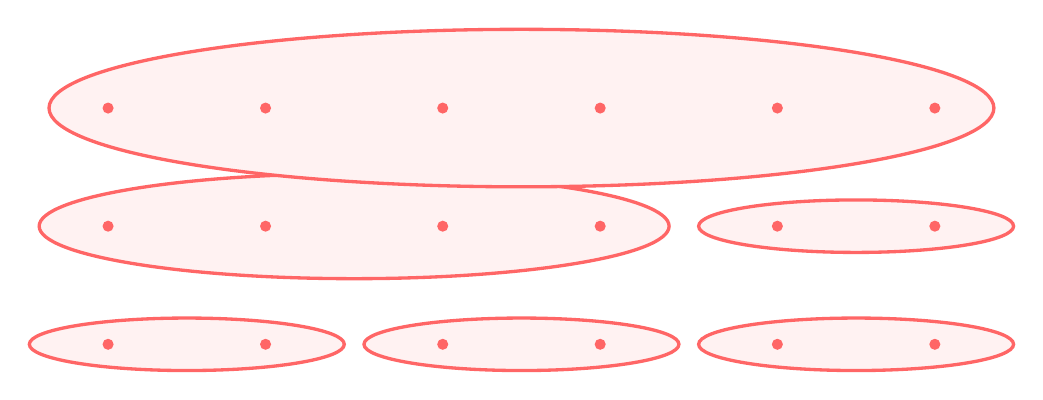
\begin{tikzpicture}
    \filldraw[color=red!60, fill=red!5, very thick](-4.25,0) ellipse (2 and 1 / 3);
    \filldraw[color=red!60, fill=red!5, very thick](0,0) ellipse (2 and 1 / 3);
    \filldraw[color=red!60, fill=red!5, very thick](4.25,0) ellipse (2 and 1 / 3);
    
    \filldraw[color=red!60, fill=red!5, very thick](-2.125,1.5) ellipse (4 and 2 / 3);
    \filldraw[color=red!60, fill=red!5, very thick](4.25,1.5) ellipse (2 and 1 / 3);
    
    \filldraw[color=red!60, fill=red!5, very thick](0,3) ellipse (6 and 1);

    \foreach \y in {0,1.5,3}
    {
        \fill[color=red!60] (-5.25,\y) circle (2pt);
        \fill[color=red!60] (-3.25,\y) circle (2pt);
        
        \fill[color=red!60] (-1,\y) circle (2pt);
        \fill[color=red!60] (1,\y) circle (2pt);
        
        \fill[color=red!60] (3.25,\y) circle (2pt);
        \fill[color=red!60] (5.25,\y) circle (2pt);
    }
    \end{tikzpicture}
    \caption{\todo Visualization of a dendogram. (... notice how this is a dendogram since the top most partition is the trivial partition)}
    \label{fig:enter-label}
\end{figure}

\section{Outputs of Clustering Schemes}

\begin{definition}{Outputs of Standard Clustering Schemes}{}
Here we define the category of outputs of \emph{standard clustering schemes}. We have:
\begin{equation*}
    \ob(\C) := \{(X, P_X): X \text{ a finite set and } P_X \in \P(X)\}
\end{equation*}
And morphisms:
\begin{equation*}
    \mor_\C((X, P_X), (Y,P_Y)) = \{f: X \to Y: P_X \refines f_*(P_Y)\}
\end{equation*}
The composition is given by the composition of maps and the identity is the identity function.
\end{definition}

\todo i think there is an intuition here about morphisms being in some sense monotonic, related to how funcitons are distance non increasing in $\gen$

\begin{definition}{Outputs of Hierarchical Clustering Schemes}{}
Now we define the outputs of \emph{hierarchical clustering schemes}. We define:
\begin{equation*}
    \ob(\C) := \{(X, \theta_X): X \text{ a finite set and } \theta_X: \R_{\geq0} \to \P(X) \text{ a quasi-dendogram}\}
\end{equation*}
And morphisms:
\begin{equation*}
    \mor_\C((X, \theta_X), (Y,\theta_Y)) = \{f: X \to Y: \forall r \in \R_{\geq0}: \theta_X(r) \refines f_*(\theta_Y(r)) \}
\end{equation*}
The composition is given by the composition of maps and the identity is the identity function.
\todo[format the equations]
\end{definition}

\section{Clustering Functors}
Finally we can define the clustering functor. For the remainder of the report we will study existences and characterizations of such objects.
\begin{definition}{Clustering Functor}{}
A \emph{clustering functor} is a functor from $\M \in \{\iso, \inj, \gen\}$ to $\A \in \{\C, \H\}$
$$\Cf : \M \longrightarrow \A.$$
Such that for the forgetful functors $\alpha, \beta$ on $\M$ and $\A$ respectively we have
\begin{equation*}
    \beta \circ \Cf = \alpha.
\end{equation*}
If $\A = \C$ then $\Cf$ is called a \emph{classical clustering functor} and if $\A = \H$ then we call it a \emph{hierarchical clustering functor}.
\end{definition}

\todo[intution about categories being invariances]

\todo[size of $\M$ inversely correlates to diversity of such functors]

\section{Excessive Clustering Functor}
\begin{definition}{Excessive Clustering Scheme}{}
A classical clustering functor $\Cf: \M \to \C$ is called \emph{excessive} if for every $(X,d) \in \ob(\M)$ and $(X,P_X) = \Cf(X,d)$ we have that for every $X_\alpha \in P_X$
\begin{equation*}
    \Cf(X_\alpha, d|_{X_\alpha \times X_\alpha}) = (X,\{X_\alpha\}).
\end{equation*}
\end{definition}
In other words if $\Cf$ is excessive it can be thought of as being nilpotent in a certain sense.

\begin{myremark}{Excessive Clustering Algorithms}{}
The notion of excessiveness exists in the more general setting of clustering alogrithms (which are not necessarily clustering functors).
\end{myremark}

\todo[reference to first chapter]
In particular there we have encountered examples of non excessive clustering algorithms.

\todo[explain why agglomerative / kmeans ... clustering is non excessive]

\todo[give an example of a excessive clustering that we have seen before]

\section{Surjective Clustering Functor}
\begin{definition}{Surjective Clustering Functor}{}
A classical clustering functor $\Cf: \M \to \C$ is called \emph{surjective} if for every finite set $X$ and every $P_X \in \P(X)$ there exists a metric $d_X$ on $X$ such that
\begin{equation*}
    \Cf(X,d_X) = (X,P_X)
\end{equation*}
\end{definition}

\todo[kmeans is not surjective, as it limits the number of classes]


\begin{proposition}{}{universality_of_surjective_functors}
Let $\mathfrak{S}: \M \to \C$ be a surjective functor. Then for any clustering functor $\Cf: \M \to \C$ there exists a functor $\Tf_\Cf: \M \to \M$ that changes the metric such that

\begin{equation*}
\Cf = \mathfrak{S} \circ \Tf_\Cf
\end{equation*}
\end{proposition}

A surprising fact about surjective clustering functors is given by the following lemma:

\begin{lemma}{}{surjective_implies_eventually_discrete}
Let $\Cf: \M \to \C$ be a surjective clustering functor and $(X,d)$ a finite metric space. Then there exists $\lambda_0, \mu_0 > 0$ such that
\begin{enumerate}
    \item $\Cf(X,\lambda \cdot d)$ is discrete for all $\lambda > \lambda_0$
    \item $\Cf(X,\mu \cdot d)$ is trivial for all $0 < \mu \le \mu_0$
\end{enumerate}
\end{lemma}

Indeed this now motivates us to define the smallest resp. largest values for which the condition in the lemma holds. This gives us:

\begin{definition}{}{}
Let $\Cf: \M \to \C$ be surjective clustering scheme. Due to the previous lemma we can define
\begin{align*}
\diam^\Cf(X) &:= \sup\{ \lambda > 0: \Cf(X,\lambda \cdot d) \text{ is trivial}\} < \infty\\
\sep^\Cf(X) &:= \inf\{ \lambda > 0: \Cf(X,\lambda \cdot d) \text{ is discrete}\} < \infty
\end{align*}
called the \emph{intrinsic separation} and \emph{diameter} of $X$. 
\end{definition}
Additionally, it is easy to check that we can use $\lambda_0 = \sep^\Cf(X)$ and $\mu_0 = \diam^\Cf(X)$ in the previous lemma.

Later we will use $\sep^\Cf(X)$ and $\diam^\Cf(X)$ but first we have to show an important property.

\begin{lemma}{}{mutliplicativity_of_intrinsic_sizes}
Let $\Cf: \M \to \C$ be surjective. Then for all $(X,d) \in \ob(\M)$ and $\lambda > 0$ we have
\begin{align*}{}{}
    \diam^\Cf(X,\lambda \cdot d) &= \lambda \cdot \diam^\Cf(X,\lambda) \\
    \sep^\Cf(X,\lambda \cdot d) &= \lambda \cdot \sep^\Cf(X,\lambda)
\end{align*}
 \end{lemma}

In the next chapters we will use the tools from this chapter to first classify classical clustering functors and then hierarchical clustering functors.